\scanpage{23}
\mspage{5}

Thus, the sub-$\unsure{\mathcal G_3|\mathfrak S_3}$-set \inserted{$X'_3$} of $X_3$ generated by $d(X_2)$ has a unique orbit with 1 \unsure{element}, namely $\{e_3\}=\{de_2\}$, all the other orbits are of cardinality 3 \deleted{and} (in the regular representation of $\unsure{\mathcal G_3|\mathfrak S_3|\deleted{\mathcal G}_3|\deleted{\mathfrak S}_3}$), and they are in one-to-one correspondence with the elements of $X_2\setminus\{e_2\}\overset{\mathrm{def}}=X_2^*$. As a $\unsure{\mathcal G_3|\mathfrak S_3}$-set $X'_3$ is written canonically
% The two X-shaped overstrokes are retained locally as live/struck alternatives; their function is unresolved.
\[
X'_3\simeq\{e_3\}\amalg\left(\unsure{\mathcal G_3|\mathfrak S_3|\deleted{\mathcal G}_3|\deleted{\mathfrak S}_3}\wedge_{\{1,\sigma_1\}}X_2^*\right),
\]
where $\{1,\sigma_1\}$ acts trivially on $X_2^*$

\margin{And we have an explicit description of $p$ on $X'_3$ via the first three of the five formulas $(*)$, \unsure{the rest} to be satisfied \unsure{being} \unsure{formal} \unsure{by these three formulas} \unsure{case|(a)}}

It remains to express
\[
X_3^*\overset{\mathrm{def}}=X_3\setminus\underbrace{X'_3}_{\unsure{\mathcal G_3|\mathfrak S_3}\cdot d(X_2)}
\]
as a $\unsure{\mathcal G_3|\mathfrak S_3}$-set, and the map induced by $p$
% One shaft with two separated complete rightward heads.
\diagram{\begin{tikzcd}[ampersand replacement=\&,column sep=large]
X_3^*\arrow[r,"p^*=p\mid X_3^*"]\arrow[r,shorten >=12pt]\&X_2
\end{tikzcd}}
satisfying
\figure{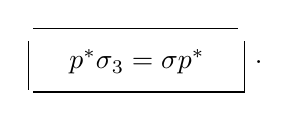
\begin{tikzpicture}[baseline=(rel.base)]
\node[inner sep=4pt] (rel) at (0,0) {$p^*\sigma_3=\sigma p^*$};
\draw[line width=.45pt] (-1.32,.43)--(1.28,.43);
\draw[line width=.45pt] (-1.38,.27)--(-1.38,-.36);
\draw[line width=.45pt] (-1.32,-.38)--(1.37,-.38)--(1.37,.27);
\node[anchor=west,inner sep=0pt] at (1.49,0) {.};
\end{tikzpicture}}

\diagram{\begin{tikzcd}[ampersand replacement=\&,column sep=large]
X_3\arrow[r,two heads,"{p,p\rho}"]\&X_2\times X_2\&\text{epimorphism}
\end{tikzcd}}

\margin{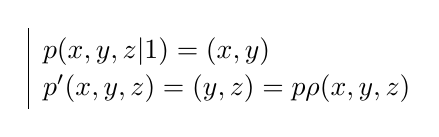
\begin{tikzpicture}[baseline=(r1.base)]
\draw[line width=.45pt] (0,.30)--(0,-.72);
\node[anchor=west,inner sep=0pt] (r1) at (.18,0) {$p(x,y,\unsure{z|1})=(x,y)$};
\node[anchor=west,inner sep=0pt] at (.18,-.47) {$p'(x,y,z)=(y,z)=p\rho(x,y,z)$};
\end{tikzpicture}}

for $\unsure{\zeta|\xi},\eta\in X_2$, $\exists\alpha\in X_3$ with
\[
p\alpha=\unsure{\zeta|\xi},\quad p\rho\alpha=\eta
\]

\margin{22}
